\chapter{File System Driver}
\label{cha:FileSystemDriver}

%----------
\section{Overview}
This documentation does not provide information about the read functionality of the driver. Also the basic concepts of a file system driver and general descriptions are not included. This information have already been given in the documentation of the continuing studies diploma thesis \cite{Ext2fuerXP}.

%----------
\section{Ext2 Write}
\subsection{General Data flow}
Whenever a user mode application or a kernel mode application requests an operation from a file system driver (FSD), the I/O Manager allocates an IRP (I/O request packet) and calls the FSD with this IRP. The FSD accesses its I/O stack location in the IRP to determine what operation (indicated by the \verb~IRP_MJ_XXX~ function code) it should carry out on the target device. The target device is represented by the device object in its designated I/O stack location and is passed with the IRP to the driver. 

\subsection{Create a new file}
An IRP\_MJ\_CREATE is sent to the FSD whenever a new file or directory is created, or when a an existing file, device, directory, or volume is being opened. Normally this IRP is sent when an application has called \verb~CreateFile()~. An IRP\_MJ\_WRITE is sent to the FSD, for example, when an application has called \verb~WriteFile()~.

\begin{figure}[H]
\begin{center}
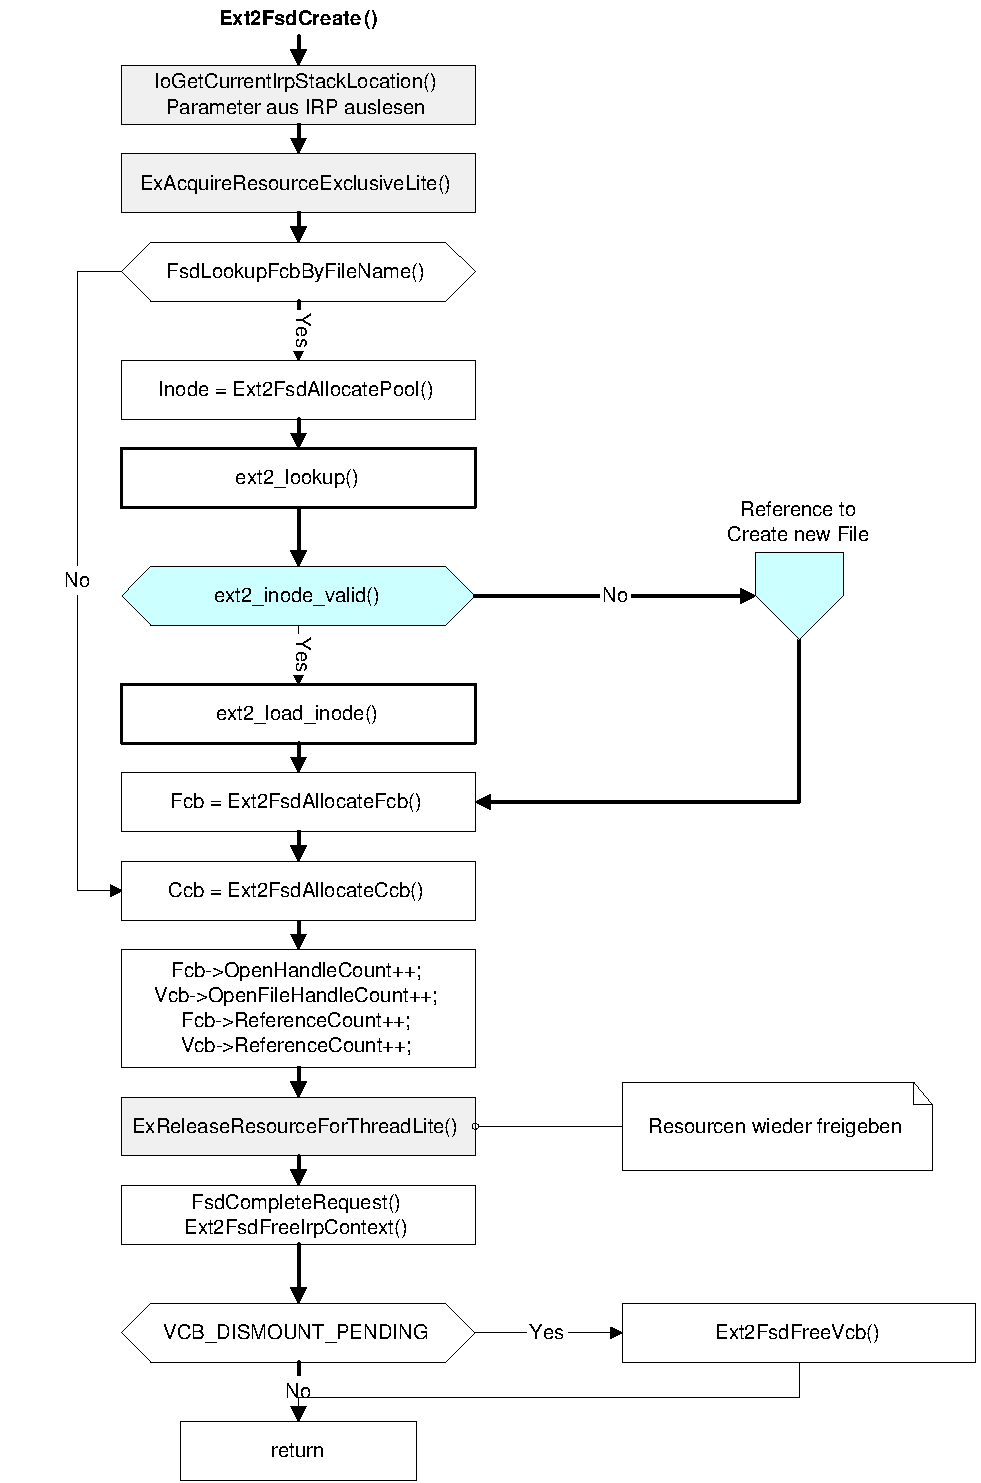
\includegraphics[height=\textheight]{./files/inc/pdf/Ext2FsdCreate}
\end{center}
\caption{\label{fig:ext2FsdCreate}Process Flow when receiving IRP\_MJ\_CREATE}
\end{figure}

\noindent
This means, whenever the FSD receives a IRP\_MJ\_CREATE, it tests if a new file needs to be created. If so, preliminary tests (file or directory name validity, flags, etc.) are made and a new Inode is created. Figure \ref{fig:ext2FsdCreate} illustrates this procedure of receiving an IRP\_MJ\_CREATE request and figure \ref{fig:ext2FsdNewFile} illustrates the process of creating a new inode in detail. The two diagrams do not describe function in detail. They only give a general overview of the basic data flow.

\begin{figure}[H]
\begin{center}
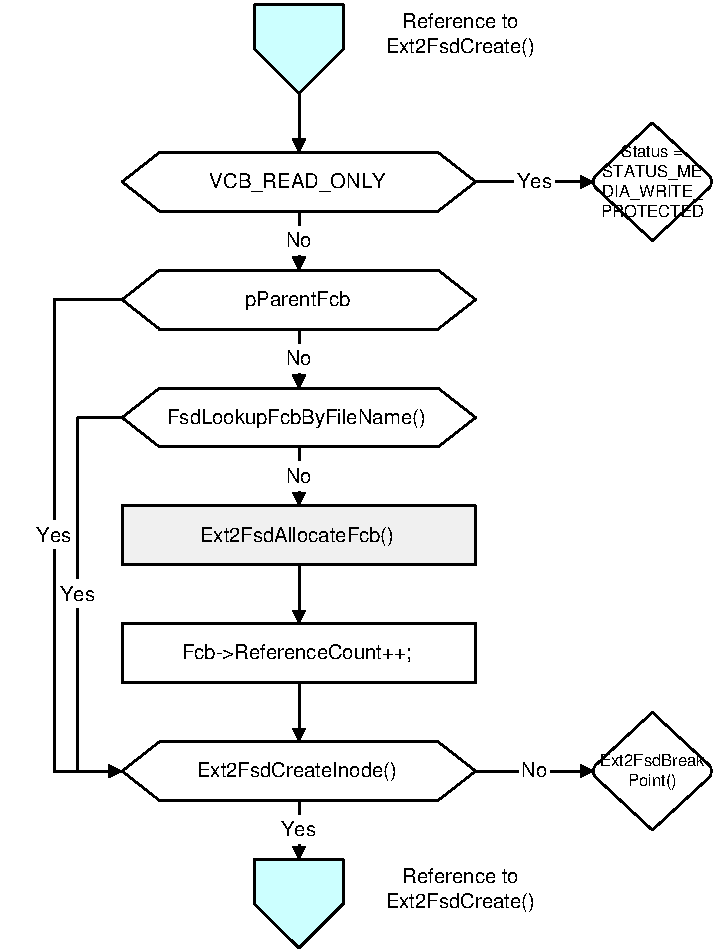
\includegraphics[height=11.5cm]{./files/inc/pdf/Ext2FsdNewFile}
\end{center}
\caption{\label{fig:ext2FsdNewFile}Process flow when creating a new inode}
\end{figure}

\noindent
Every function in the above two diagrams are subject to describe in more detail. This has been done in the code documentation in part \ref{par:implementation}. For even more details please consult the code.
